\documentclass{article}
\usepackage[utf8]{inputenc}
% are all of these packages really necessary?
% no.
% i'm just too lazy to only grab the packages i want for a specific
% document, so i just glob all of my most commonly used packages together
% this is bad practice.
\usepackage{amsmath,amsthm,amssymb,amsfonts, fancyhdr, color, comment, graphicx, environ, mdframed, soul, calc, enumitem, mdframed, xcolor, geometry, empheq, mathtools, tikz, pgfplots, caption, subcaption, hyperref,multicol, textcomp, gensymb}

\usetikzlibrary{external}
\tikzexternalize[prefix=tikz/,optimize command away=\includepdf]

%tikzpicture
\usepackage{tikz}
\usepackage{scalerel}
\usepackage{pict2e}
\usepackage{tkz-euclide}
\usetikzlibrary{calc}
\usetikzlibrary{patterns,arrows.meta}
\usetikzlibrary{shadows}
\usetikzlibrary{external}

%pgfplots
\usepackage{pgfplots}
\pgfplotsset{compat=newest}
\usepgfplotslibrary{statistics}
\usepgfplotslibrary{fillbetween}
\usepgfplotslibrary{polar}

\tikzset{external/export=true}
\pgfplotsset{
    standard/.style={
    axis line style = thick,
    trig format=rad,
    enlargelimits,
    axis x line=middle,
    axis y line=middle,
    enlarge x limits=0.15,
    enlarge y limits=0.15,
    every axis x label/.style={at={(current axis.right of origin)},anchor=north west},
    every axis y label/.style={at={(current axis.above origin)},anchor=south east}
    }
}
\newcommand*\widefbox[1]{\fbox{\hspace{2em}#1\hspace{2em}}}
% Command "alignedbox{}{}" for a box within an align environment
% Source: http://www.latex-community.org/forum/viewtopic.php?f=46&t=8144
\newlength\dlf  % Define a new measure, dlf
\newcommand\alignedbox[2]{
% Argument #1 = before & if there were no box (lhs)
% Argument #2 = after & if there were no box (rhs)
&  % Alignment sign of the line
{
\settowidth\dlf{$\displaystyle #1$}  
    % The width of \dlf is the width of the lhs, with a displaystyle font
\addtolength\dlf{\fboxsep+\fboxrule}  
    % Add to it the distance to the box, and the width of the line of the box
\hspace{-\dlf}  
    % Move everything dlf units to the left, so that & #1 #2 is aligned under #1 & #2
\boxed{#1 #2}
    % Put a box around lhs and rhs
}
}

\hypersetup{
    colorlinks=true,
    linkcolor=blue,
    filecolor=magenta,      
    urlcolor=cyan,
    pdftitle={Final Review Solutions},
    pdfpagemode=UseOutlines,
    bookmarksopen=true,
    pdfauthor={Christina Phan}
}
\newcommand{\lrp}[1]{\left( #1 \right)}
\newcommand{\abs}[1]{\left\vert #1 \right\vert}
\newcommand{\lra}[1]{\left\langle #1 \right\rangle}
\newcommand{\lrb}[1]{\left[ #1 \right]}
\newcommand{\norm}[1]{\left\lVert #1 \right\rVert}
\newcommand{\iintR}[0]{\iint\limits_{R}}
\renewcommand{\u}[0]{\mathbf{u}}
\renewcommand{\i}[0]{\mathbf{{i}}}
\renewcommand{\j}[0]{\mathbf{{j}}}
\renewcommand{\k}[0]{\mathbf{{k}}}
\newcommand{\T}[0]{\mathbf{T}}
\newcommand{\N}[0]{\mathbf{N}}
\newcommand{\B}[0]{\mathbf{B}}
\renewcommand{\r}[0]{\mathbf{r}}
\renewcommand{\a}[0]{\mathbf{a}}
\renewcommand{\v}[0]{\mathbf{v}}
\newcommand{\F}[0]{\mathbf{F}}
\newcommand{\G}[0]{\mathbf{G}}
\newcommand{\n}[0]{{\mathbf{n}}}
\newcommand{\eqq}[0]{\stackrel{?}{=}}
\renewcommand{\arraystretch}{1.25}

\geometry{letterpaper, portrait, margin=1in}
\renewcommand{\footrulewidth}{0.8pt}
\setlength\parindent{0pt}
\pagestyle{fancy}
\lhead{Christina Phan}
\rhead{MAT 21D} 
\chead{\textbf{Final Review Solutions}}

\newcommand{\Solution}{\textit{Solution}}
\pgfplotsset{compat=1.18}
\begin{document}

\phantomsection
\addcontentsline{toc}{section}{Problem 1}\textbf{Problem 1}

Integrate $f(x,y)=\sqrt{x^2+y^2}$ over $\r(t)=\lra{\cos t + t\sin t, \sin t - t\cos t}$, $0\leq t\leq \sqrt{3}$.

\Solution

\textit{Similar problems in Homework 11, Problem 1; Campuswire \#48}

Since $\r(t)=\lra{\cos t + t\sin t, \sin t - t\cos t}$,
\begin{align*}
f(\lrp{\r(t)})&=\sqrt{\lrp{\cos t + t\sin t}^2 + (\sin t - t\cos t)^2}\\
&=\sqrt{\lrp{\cos^2t + 2t\sin t \cos t + t^2\sin^2 t}+\lrp{\sin^2 t - 2t\sin t\cos t+t^2\cos^2 t}}\\
&=\sqrt{\cos^2 t +\sin^2 t + t^2\sin^2 t + t^2\cos ^ 2 t }\\
&=\sqrt{1 + t^2\lrp{\sin ^2 t + \cos ^ 2 t}}\tag{$\cos ^2 t + \sin ^2 t = 1$}\\
&=\sqrt{1 + t^2}\tag{$\sin ^2 t + \cos ^2 t + 1$}\\
    \r'(t)&=\lra{-\sin t + \sin t + t\cos t, \cos t - \cos t + t\sin t}=\lra{t\cos t, t \sin t}\\
    \norm{\r'(t)}&=\sqrt{(t\cos t)^2+(t\sin t)^2}=\sqrt{t^2\cos^2 t + t^2\sin^2 t}=\sqrt{t^2(\cos ^2 t + \sin ^2 t)}=\sqrt{t^2(1)}=t\tag{$\cos^2 t+ \sin^2 t = 1$, $t\geq 0$}
\end{align*}
Let's evaluate the integral.
\begin{align*}
   \int_C f(x,y)\,ds&= \int_C \sqrt{x^2+y^2}\,ds\\
   &=\int_0^{\sqrt{3}}\lrp{\sqrt{1+t^2}}\lrp{t}\,dt\\
   &=\lrb{\frac{1}{3}(1+t^2)^{3/2}}_0^{\sqrt{3}}\tag{or do $u$-sub, $u=1+t^2$}\\
   &=\lrp{\frac{1}{3}\lrp{1+\lrp{\sqrt{3}}^2}^{3/2}}-\lrp{\frac{1}{3}(1+0^2)^{3/2}}\\
   &=\lrp{\frac{1}{3}(1+3)^{3/2}}-\lrp{\frac{1}{3}(1)^{3/2}}\\
   &=\lrp{\frac{1}{3}(8)}-\lrp{\frac{1}{3}}\tag{$4^{3/2}=\lrp{\sqrt{4}}^3=2^3$}\\
   &=\boxed{\frac{7}{3}}
\end{align*}

\phantomsection
\addcontentsline{toc}{section}{Problem 2}\textbf{Problem 2}

Evaluate the integral $\displaystyle \int_{(-1,1,1)}^{(4,-3,0)}\frac{dx+dy+dz}{\sqrt{x+y+z}}$.

\Solution

\textit{Similar problems in Homework 14, Problem 2 and Homework 15, Problem 3; Campuswire \#52 and Campuswire \#55}

Recall that the Fundamental Theorem for Line Integrals states that if $\F$ is a conservative vector field with potential function $f$,
\begin{equation*}
    \int_{C}\F\cdot d\r=f\lrp{\r(b)}=f\lrp{\r(a)}
\end{equation*}
We can slightly rewrite our integral to become
\begin{equation*}
    \int_{(-1,1,1)}^{(4,-3,0)}\frac{dx+dy+dz}{\sqrt{x+y+z}}=\int_{(-1,1,1)}^{(4,-3,0)}\frac{1}{\sqrt{x+y+z}}\,dx+\frac{1}{\sqrt{x+y+z}}\,dy+\frac{1}{\sqrt{x+y+z}}\,dz
\end{equation*}
Let $\F(x,y,z)=\lra{\frac{1}{\sqrt{x+y+z}},\frac{1}{\sqrt{x+y+z}},\frac{1}{\sqrt{x+y+z}}}$ where $\F=\nabla f$.

It looks like $f(x,y,z)=2\sqrt{x+y+z}$. We can verify this by checking if $\nabla f = \F$.
\begin{align*}
    \nabla f &= \lra{\frac{2}{2\sqrt{x+y+z}},\frac{2}{2\sqrt{x+y+z}},\frac{2}{2\sqrt{x+y+z}}}\\
    &=\lra{\frac{1}{\sqrt{x+y+z}},\frac{1}{\sqrt{x+y+z}},\frac{1}{\sqrt{x+y+z}}}\\
    &=\F
\end{align*}
Since $\nabla f= \F$, we know $\F$ is conservative.

Therefore,
\begin{align*}
    \int_{(-1,1,1)}^{(4,-3,0)}\frac{dx+dy+dz}{\sqrt{x+y+z}}&=\lrb{f(x,y,z)}_{(-1,1,1)}^{(4,-3,0)}\\
    &=f(4,-3,0)=f(-1,1,1)\\
    &=\lrp{2\sqrt{4+(-3)+0}}-\lrp{2\sqrt{(-1)+1+1}}\\
    &=\lrp{2\sqrt{1}}-\lrp{2\sqrt{1}}\\
    &=\lrp{2}-\lrp{2}\\
    &=\boxed{0}
\end{align*}
\textbf{Note}

You could have also done the formal method of proving that $\F$ is conservative (do the component test and a bunch of antiderivatives).

The formal method, while valid, takes up a lot of time. I would only do it if you're speedy :)

\phantomsection
\addcontentsline{toc}{section}{Problem 3}\textbf{Problem 3}

Evaluate $\displaystyle \oint_C 8x\sin y\,dx-8y\cos x\,dy$, where $C$ is the square cut from the first quadrant by the lines $x=\dfrac{\pi}{2}$ and $y=\dfrac{\pi}{2}$.

\Solution

\textit{Similar problems in Homework 16, Problem 1; Campuswire \#57}

Recall that Green's Theorem states that
\begin{align*}
    \int_C \mathbf{F} \cdot d\mathbf{r} = \iint_R \frac{\partial N}{\partial x} - \frac{\partial M}{\partial y}\,dA
\end{align*}
Let $\F=\lra{8x\sin y, -8y\cos x}$ then,
\begin{align*}
 M=8x\sin y&\implies \frac{\partial M}{\partial y}=8x\cos y\\
  N=-8y\cos x&\implies  \frac{\partial N}{\partial x}= 8y \sin x
\end{align*}
Our region $R$ is given in the problem. Our region is the square consisting of $x=0$, $x=\dfrac{\pi}{2}$, $y=0$, and $y=\dfrac{\pi}{2}$.

Our lower and upper bounds for $y$ are $y=0$ and $y=\dfrac{\pi}{2}$, respectively.

Our lower and upper bounds for $x$ are $x=0$ and $x=\dfrac{\pi}{2}$, respectively.

Let's evaluate the integral.
\begin{align*}
    \oint_C \F\cdot d\r&=\oint_C 8x\sin y\,dx-8y\cos x\,dy\\
    &=\int_0^{\pi/2}\int_0^{\pi/2} 8y\sin x - 8x\cos y\,dy\,dx\\
    &=\int_0^{\pi/2}\lrb{4y^2\sin x - 8x\sin y}_0^{\pi/2}\,dx\\
    &=\int_0^{\pi/2}\lrp{4\lrp{\frac{\pi}{2}}^2\sin x-8x \sin\frac{\pi}{2}}-\lrp{4(0)^2\sin x - 8x\sin 0}\,dx\\
    &=\int_0^{\pi/2}\lrp{4\lrp{\frac{\pi^2}{4}}\sin x - 8x}-\lrp{0-0}\,dx\\
    &=\int_0^{\pi/2}\pi^2\sin x - 8x\,dx\\
    &=\lrb{-\pi^2 \cos x-4x^2}_0^{\pi/2}\\
    &=\lrp{-\pi^2 \cos \frac{\pi}{2}-4\lrp{\frac{\pi}{2}}^2}-\lrp{-\pi^2 \cos 0 -4(0)^2}\\
    &=\lrp{-\pi^2 (0)-4\lrp{\frac{\pi^2}{4}}}-\lrp{-\pi^2(1)-0}\\
    &=\lrp{-\pi^2}-\lrp{-\pi^2}\\
    &=\boxed{0}
\end{align*}
\phantomsection
\addcontentsline{toc}{section}{Problem 4}\textbf{Problem 4}

Find the area of the elliptical region cut from the plane $x+y+z=1$ by the cylinder $x^2+y^2=1$.

\Solution

\textit{Similar problems in Homework 18, Problem 1; Campuswire \#68}

Recall that if a surface is given by a function $g(x,y,z)=c$ that defines $z$ implicitly as a function of $x$ and $y$, then the area of surface is
\begin{equation*}
    S=\iint_R \frac{\norm{\nabla g}}{\left| g_z\right|}\,dA
\end{equation*}
Let $g(x,y,z)=x+y+z=1$ where $z$ is a function implicitly defined by $x$ and $y$.

Let's find $\displaystyle \frac{\norm{\nabla g}}{\left|g_z\right|}$.
\begin{align*}
    \nabla g &= \lra{1,1,1}\\
    g_z &= 1\\
    \frac{\norm{\nabla g}}{\left|g_z\right|}&=\frac{\sqrt{1^2+1^2+1^2}}{\left|1\right|}=\sqrt{3}
\end{align*}
Let's find the region $R$ that we're integrating over.

The problem tells us that we're bounded by the cylinder $x^2+y^2=1$.

Graphically, the shadow on the $xy$-plane looks like
 \begin{center}
\resizebox{5cm}{!}{
    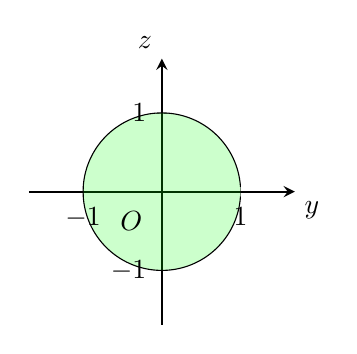
\begin{tikzpicture}
    \begin{axis}[standard,
            xtick={-1,1},
            ytick={-1,1},
            samples=1000,
            xlabel={$y$},
            ylabel={$z$},
          xmin=-1.3,xmax=1.3,           ymin=-1.3,ymax=1.3,
            x=1cm,
            y=1cm/1,
           ]

    \node[anchor=center,label=south west:$O$] at (axis cs:0,0){};
\addplot[name path=F,domain={-1:1}]{sqrt(1-x^2)};
\addplot[name path=G,domain={-1:1}]{-sqrt(1-x^2)};
\addplot[fill=green, fill opacity=0.2] fill between [of=F and G, soft clip={domain=-1:1}];
    \end{axis}
    \end{tikzpicture}
}
\end{center}
The cylinder looks like a good candidate for switching to polar. Don't forget since we’re switching to
polar, we need our Jacobian $r$.

The Jacobian is necessary because we are going from our original $x$, $y$ coordinates to $r$, $\theta$ coordinates.

Based on the graph above,

Our lower and upper bounds for $r$ are $r=0$ and $r=1$, respectively.
Our lower and upper bounds for $\theta$ are $\theta=0$ and $\theta=2\pi$, respectively.

Let's evaluate the integral.
\begin{align*}
    S&=\int_0^{2\pi}\int_0^1 \lrp{\sqrt{3}}r\,dr\,d\theta\tag{don't forget our Jacobian $r$!}\\
    &=\int_0^{2\pi}\lrb{\frac{\sqrt{3}}{2}r^2}_0^1\,d\theta\\
    &=\int_0^{2\pi}\frac{\sqrt{3}}{2}\,d\theta\\
    &=\lrb{\frac{\sqrt{3}}{2}\theta}_0^{2\pi}\\
    &=\frac{\sqrt{3}}{2}\lrp{2\pi}\\
    &=\boxed{\sqrt{3}\pi}
\end{align*}
\phantomsection
\addcontentsline{toc}{section}{Problem 5 (Parts)}\textbf{Problem 5 (Parts)}

Find a parameterization for the surface:

\textit{Similar problems in Homework 17, Problem 1; Campuswire \#64}

\phantomsection
\addcontentsline{toc}{subsection}{5(a)}\textbf{(a)} The portion of the sphere $x^2+y^2+z^2=36$ between $z=-3$ and $z=3\sqrt{3}$.

\Solution

The portion of the \textit{sphere}... let's use spherical coordinates!

Since we have a sphere of radius $\sqrt{36}=6$, in spherical coordinates,
\begin{align*}
    x &= 6\sin\phi\cos\theta\\
    y&=6\sin\phi\sin\theta\\
    z&=6\cos\phi
\end{align*}
Let's find the bounds for $\phi$ and $\theta$.

For $\phi$,

Since $-3\leq z \leq 3\sqrt{3}$,
\begin{align*}
    -3\leq &z \leq 3\sqrt{3}\\
    -3 \leq &6\cos \phi \leq 3\sqrt{3}\tag{in spherical, $z=\rho\cos\phi$; we know $\rho=\sqrt{36}=6$}\\
    -\frac{1}{2}\leq &\cos \phi \leq \frac{\sqrt{3}}{2}\\
    \implies \frac{\pi}{6}\leq & \phi \leq \frac{2\pi}{3}\tag{see note}
\end{align*}
\textbf{Note}

We need to be a little careful when jumping from $\displaystyle -\frac{1}{2}\leq \cos \phi \leq \frac{\sqrt{3}}{2}$ to $\displaystyle \frac{\pi}{6}\leq \phi \leq \frac{2\pi}{3}$. Don't forget that $\phi$ is \textbf{always} bounded between $\phi=0$ and $\phi=\pi$. We know $\cos^{-1}\lrp{-\dfrac{1}{2}}=\dfrac{2\pi}{3}$ and $\cos^{-1}\dfrac{\sqrt{3}}{2}=\dfrac{\pi}{6}$, so our $\phi$ angle must be in between those two values.

For $\theta$,

Since we're going around the entire sphere, our lower and upper bounds for $\theta$ are $\theta=0$ and $\theta=2\pi$, respectively.

Our final answer is
\begin{equation}
    \boxed{\r(\phi,\theta)=\lra{6\sin\phi\cos\theta,6\sin\phi\sin\theta, 6\cos\phi}}\tag{$\displaystyle\frac{\pi}{6}\leq \phi\leq \frac{2\pi}{3}$, $\displaystyle 0\leq \theta\leq 2\pi$}
\end{equation}

\phantomsection
\addcontentsline{toc}{subsection}{5(b)}\textbf{(b)} The cone $z=1+\sqrt{x^2+y^2}$, $z\leq 3$

\Solution

The $x^2+y^2$ gives off cylindrical coordinate vibes.

In cylindrical coordinates,
\begin{align*}
    x&=r\cos\theta\\
    y&=r\sin\theta\\
    z&=1+\sqrt{x^2+y^2}\\
   &= 1+\sqrt{r^2\cos^2\theta+r^2\sin^2\theta}\\
    &=1+\sqrt{r^2(\cos^2\theta+\sin^2\theta)}\\
    &=1+\sqrt{r^2}\tag{$\cos^2\theta+\sin^2\theta=1$}\\
    &=1+r\tag{$r\geq 0$ always}
\end{align*}
Let's find the bounds for $r$ and $\theta$.

For $r$,

The smallest possible value of $z$ is $z=1$ since $z=1+\sqrt{0^2+0^2}=1$ (the smallest $\sqrt{x^2+y^2}$ gets is $\sqrt{x^2+y^2}=0$). We already know the largest possible values of $z$ is $z=3$ since the problem tells us that $z\leq 3$.

Since $1\leq z \leq 3$,
\begin{align*}
    1 \leq & z \leq 3\\
    1 \leq & 1 + r \leq 3\\
    0 \leq & r \leq 2 \\
\end{align*}
For $\theta$,

Since we're going around the entire cone, our lower and upper bounds for $\theta$ are $\theta=0$ and $\theta=2\pi$, respectively.

Our final answer is
\begin{equation*}
    \boxed{\r(r,\theta)=\lra{r\cos\theta, r\sin\theta, 1+r}}\tag{$0\leq r\leq 2$, $0\leq \theta\leq2\pi$}
\end{equation*}
\phantomsection
\addcontentsline{toc}{section}{Problem 6}\textbf{Problem 6}

Find the area of the surface $\r(u,v)=\lra{u+v,u-v,v}$, $0\leq u\leq 1$, $0\leq v\leq 1$.

\Solution

\textit{Similar problems in Homework 17, Problem 2; Campuswire \#64}

Recall that surface area is
\begin{align*}
    S=\iint_R \norm{\frac{\partial \r}{\partial u}\times \frac{\partial \r}{\partial v}}\,dA
\end{align*}
Let's find what $\displaystyle \norm{\frac{\partial \r}{\partial u}\times \frac{\partial \r}{\partial v}}$ is.
\begin{align*}
    \frac{\partial \r}{\partial u}&=\lra{1, 1, 0}\\
    \frac{\partial \r}{\partial v}&=\lra{1,-1,1}\\
    \frac{\partial \r}{\partial u}\times   \frac{\partial \r}{\partial v}&=\begin{vmatrix}\i & \j & \k \\ 1 & 1 & 0\\ 1 & -1 & 1\end{vmatrix}\\
      &=\lrp{1 - 0}\i-\lrp{1 - 0}\j + \lrp{-1-1}\k\\
      &=\lrp{1}\j - \lrp{1}\j + \lrp{-2}\k\\
      &=\lra{1,-1,-2}\\
    \norm{\frac{\partial \r}{\partial u}\times   \frac{\partial \r}{\partial v}}&=\sqrt{1^2+(-1)^2+(-2)^2}=\sqrt{1+1+4}=\sqrt{6}  
\end{align*}
Let's evaluate the integral.
\begin{align*}
    S&=\int_0^1\int_0^1 \sqrt{6}\,du\,dv\\
    &=\int_0^1 \lrb{\sqrt{6}u}_0^1\,dv\\
    &=\int_0^1 \sqrt{6}\,dv\\
    &=\lrb{\sqrt{6}v}_0^1\\
    &=\boxed{\sqrt{6}}
\end{align*}
\phantomsection
\addcontentsline{toc}{section}{Problem 7}\textbf{Problem 7}

Find the area of the cap cut from the paraboloid $y^2+z^2=3x$ by the plane $x=1$.

\Solution

\textit{Similar problems in Homework 18, Problem 2; Campuswire \#68}

Recall that if a surface is given by a function $g(x,y,z)=c$ that defines $z$ implicitly as a function of $x$ and $y$, then the area of surface is
\begin{equation*}
    S=\iint_R \frac{\norm{\nabla g}}{\left| g_x\right|}\,dA
\end{equation*}
Let $g(x,y,z)=-3x+y^2+z^2=0$ where $x$ is a function implicitly defined by $y$ and $z$ ($y^2+z^2=3x\implies -3x+y^2+z^2=0$.)

Let's find $\displaystyle \frac{\norm{\nabla g}}{\left|g_x\right|}$.
\begin{align*}
    \nabla g &=\lra{-3,2y,2z}\\
    g_x &=-3\\
    \frac{\norm{\nabla g}}{\left|g_x\right|}&=\frac{\sqrt{(-3)^2+(2y)^2+(2z)^2}}{\left|-3\right|}=\frac{\sqrt{9+4y^2+4z^2}}{3}=\frac{\sqrt{9+4(y^2+z^2)}}{3}
\end{align*}

Let's find the region $R$ that we're integrating over.

Our region is the shadow of the surface in the $yz$-plane. 

Since $x=1$, $y^2+z^2=3(1)=3$.

Our region is a circle of radius $\sqrt{3}$.
\begin{center}
\resizebox{4cm}{!}{
    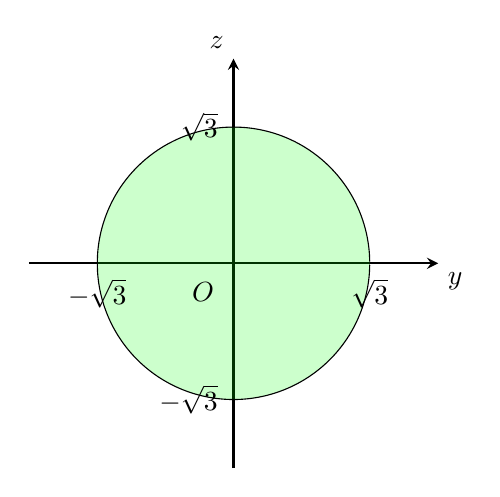
\begin{tikzpicture}
    \begin{axis}[standard,
            xtick={-1.73,1.73},
            ytick={-1.73,1.73},
            samples=1000,
            xlabel={$y$},
            ylabel={$z$},
          xmin=-2,xmax=2,           ymin=-2,ymax=2,
            x=1cm,
            y=1cm/1,        xticklabels={$-\sqrt{3}$, $\sqrt{3}$},
            yticklabels={$-\sqrt{3}$, $\sqrt{3}$}
           ]

    \node[anchor=center,label=south west:$O$] at (axis cs:0,0){};
\addplot[name path=F,domain={-1.73:1.73}]{sqrt(1.73^2-x^2)};
\addplot[name path=G,domain={-1.73:1.73}]{-sqrt(1.73^2-x^2)};
\addplot[fill=green, fill opacity=0.2] fill between [of=F and G, soft clip={domain=-1.73:1.73}];
    \end{axis}
    \end{tikzpicture}
}
\end{center}
Since our region is a circle, it might be a good idea to switch to polar where $y=r\cos\theta$ and $z=r\sin\theta$. Don't forget that since we're switching to polar, we need our Jacobian $r$.

In polar,
\begin{equation*}
    \frac{\norm{\nabla g}}{\left|g_x\right|}=\frac{\sqrt{9+4(y^2+z^2)}}{3}=\frac{\sqrt{9+4r^2}}{3}
\end{equation*}
Based on the graph above,

Our lower and upper bounds for $r$ are $r=0$ and $r=\sqrt{3}$, respectively.

Our lower and upper bounds for $\theta$ are $\theta=0$ and $\theta=2\pi$, respectively.

Let's evaluate the integral.
\begin{align*}
    S&=\int_0^{2\pi}\int_0^{\sqrt{3}} \lrp{\frac{\sqrt{9+4r^2}}{3}}r\,dr\,d\theta\tag{don't forget our Jacobian $r$!}\\
    &=\int_0^{2\pi}\int_0^{\sqrt{3}}\frac{1}{3}r\sqrt{9+4r^2}\,dr\,d\theta\\
    &u=9+4r^2\hspace{2em}du=8r\,dr\\
    &u(0)=9\hspace{2em}u(\sqrt{3})=21\\
    &=\int_0^{2\pi}\int_9^{21}\frac{1}{24}\sqrt{u}\,du\,d\theta\\
    &=\int_0^{2\pi}\lrb{\frac{1}{36}u^{3/2}}_9^{21}\,d\theta\\
    &=\int_0^{2\pi}\frac{1}{36}(21)^{3/2}-\frac{1}{36}(9)^{3/2}\,d\theta\\
    &=\lrb{\lrp{\frac{1}{36}(21)^{3/2}-\frac{1}{36}(9)^{3/2}}\theta}_0^{2\pi}\\
    &=\lrp{\frac{1}{36}(21)^{3/2}-\frac{1}{36}(9)^{3/2}}\lrp{2\pi}\\
    &=\lrp{\frac{1}{18}(21)^{3/2}-\frac{1}{18}(9)^{3/2}}\pi\\
    &=\lrp{\frac{1}{18}(21)(21)^{1/2}-\frac{1}{18}(9)(9)^{1/2}}\pi\\
    &=\lrp{\frac{1}{6}(7)(21)^{1/2}-\frac{1}{2}(1)(3)}\pi\\
    &=\boxed{\lrp{\frac{7\sqrt{21}}{6}-\frac{3}{2}}\pi}
\end{align*}
\phantomsection
\addcontentsline{toc}{section}{Problem 8}\textbf{Problem 8}

Find the surface area of the helicoid $\r(r,\theta)=\lra{r\cos\theta, r\sin\theta,\theta}$, $0\leq \theta\leq 2\pi$, $0\leq r\leq 1$ and then evaluate $\displaystyle\iint_S\sqrt{x^2+y^2+1}\,d\sigma$.

\Solution

\textit{Similar problems in Homework 17, Problem 2 and Homework 19, Problem 1; Campuswire \#64 and Campuswire \#80}

\phantomsection
\addcontentsline{toc}{subsection}{Surface Area}\textbf{Surface Area}

Recall that surface area is
\begin{align*}
    S=\iint_R \norm{\frac{\partial \r}{\partial u}\times \frac{\partial \r}{\partial v}}\,dA
\end{align*}
Let's have $u=r$ and $v=\theta$.

Let's find what $\displaystyle \norm{\frac{\partial \r}{\partial r}\times \frac{\partial \r}{\partial \theta}}$ is. 

Since $\r(r,\theta)=\lra{r\cos\theta, r\sin\theta,\theta}$,
\begin{align*}
    \frac{\partial \r}{\partial r}&=\lra{\cos\theta, \sin\theta, 0}\\
    \frac{\partial \r }{\partial \theta}&=\lra{-r\sin\theta, r\cos\theta, 1}\\
    \frac{\partial \r}{\partial r}\times \frac{\partial \r}{\partial \theta}&=\begin{vmatrix}\i & \j & \k \\ \cos\theta& \sin \theta & 0\\ -r\sin\theta & r\cos\theta & 1\end{vmatrix}\\
    &=\lrp{\sin\theta - 0}\i -\lrp{\cos\theta - 0}\j + \lrp{r\cos^2\theta + r\sin^2\theta}\k\\
    &=\lrp{\sin\theta}\i-\lrp{\cos\theta}+\lrp{r\lrp{\cos^2\theta+\sin^2\theta}}\k\\
    &=\lrp{\sin\theta}\i-\lrp{\cos\theta}+\lrp{r}\k\tag{$\cos^2\theta+\sin^2\theta=1$}\\
    &=\lra{\sin\theta,-\cos\theta, r}\\
    \norm{\frac{\partial \r}{\partial r}\times \frac{\partial \r}{\partial \theta}}&=\sqrt{\lrp{\sin\theta}^2+\lrp{-\cos\theta}^2+r^2}=\sqrt{\sin^2\theta+\cos^2\theta+r^2}=\sqrt{1+r^2}\tag{$\sin^2\theta+\cos^2\theta=1$}
\end{align*}
Let's evaluate the surface area integral.

Note that since we already parameterized our surface in terms of $r$ and $\theta$, we \textbf{do not} need to throw in our Jacobian $r$. We already are in polar. We're not trying to switch over to polar
\begin{align*}
    S&=\int_0^{2\pi}\int_0^1\sqrt{{1+r^2}}\,dr\,d\theta\\
   &=\int_0^{2\pi}\lrb{\frac{1}{2}r\sqrt{1+r^2}+\frac{1}{2}\ln\lrp{r+\sqrt{1+r^2}}}_0^1\,d\theta\tag{see note}\\
   &r=\tan\hat{\theta}\hspace{2em}dr=\sec^2\hat{\theta}\,d\hat{\theta}\\
   &0=\tan\hat{\theta}\implies \hat{\theta}=0\\
   &1=\tan\hat{\theta}\implies \hat{\theta}=\frac{\pi}{4}\\
   &=\int_0^{2\pi}\int_0^{\pi/4}\sqrt{1+\tan^2 \hat{\theta}}\lrp{\sec^2 \hat{\theta}}\,d\hat{\theta}\\
   &=\int_0^{2\pi}\int_0^{\pi/4}\sqrt{\sec^2 \hat{\theta}}\sec^2\hat{\theta}\,d\hat{\theta}\tag{$1+\tan^2\hat{\theta}=\sec^2\hat{\theta}$}\\
   &=\int_0^{2\pi}\int_0^{\pi/4}\lrp{\sec \hat{\theta}}\lrp{\sec^2\hat{\theta}}\,d\hat{\theta}\tag{ok to drop abs since $0\leq \hat{\theta}\leq \dfrac{\pi}{4}$}\\
   &=\int_0^{2\pi}\int_0^{\pi/4}\sec^3\hat{\theta}\,d\hat{\theta}\\
   &=\int_0^{2\pi}\lrb{\frac{1}{2}\lrp{\sec \hat{\theta}\tan\hat{\theta}+\ln\left|\sec \hat{\theta}+\tan \hat{\theta}\right|}}_0^{\pi/4}\,d\theta\tag{see note}\\
   &=\int_0^{2\pi}\frac{1}{2}\lrp{\sec\frac{\pi}{4}\tan\frac{\pi}{4}+\ln\left|\sec\frac{\pi}{4}+\tan\frac{\pi}{4}\right|}-\frac{1}{2}\lrp{\sec 0\tan 0 +\ln\left|\sec 0 +\tan 0\right|}\,d\theta\\
   &=\int_0^{2\pi}\frac{1}{2}\lrp{(\sqrt{2})(1)+\ln\left|\sqrt{2}+1\right|}-\frac{1}{2}\lrp{(1)(0)+\ln\left|1+0\right|}\,d\theta\\
   &=\int_0^{2\pi}\frac{1}{2}\lrp{\sqrt{2}+\ln\left|\sqrt{2}+1\right|}-\frac{1}{2}\lrp{0+0}\,d\theta\\
   &=\int_0^{2\pi}\frac{1}{2}\lrp{\sqrt{2}+\ln\lrp{\sqrt{2}+1}}\,d\theta\tag{ok to drop abs since $\sqrt{2}+1\geq 0$}\\
   &=\lrb{\frac{1}{2}\lrp{\sqrt{2}+\ln\lrp{\sqrt{2}+1}}\theta}_0^{2\pi}\\
   &=\frac{1}{2}\lrp{\sqrt{2}+\ln\lrp{\sqrt{2}+1}}\lrp{2\pi}\\
   &=\lrp{\sqrt{2}+\ln(1+\sqrt{2})}\pi
\end{align*}
\textbf{Note}

The $\displaystyle \int \sec^3 \hat{\theta}\,d\hat{\theta}$ integral is a very common integration by parts integral given back in MAT 21B (integral calculus).
\begin{align*}
    u=\sec \hat{\theta} &\hspace{2em}dv=\sec^2 \hat{\theta}\,d\hat{\theta}\\
    du=\sec\hat{\theta}\tan\hat{\theta}\,d\hat{\theta}&\hspace{2em}v=\tan \hat{\theta}\\
    \int\sec^3 \hat{\theta}\,d\hat{\theta}&=\sec\hat{\theta}\tan\hat{\theta}-\int \sec\hat{\theta}\tan^2\hat{\theta}\,d\hat{\theta}\\
    &=\sec \hat{\theta}\tan\hat{\theta}-\int \sec\hat{\theta}\lrp{\sec^2 \hat{\theta}-1}\,d\hat{\theta}\tag{$\tan^2\hat{\theta}=\sec^2\hat{\theta}-1$}\\
    &=\sec\hat{\theta}\tan\hat{\theta}-\int \sec^3 \hat{\theta} - \sec \hat{\theta}\,d\hat{\theta}\\
    &=\sec\hat{\theta}\tan\hat{\theta}-\lrp{\int \sec^3 \hat{\theta}\,d\hat{\theta} - \int \sec \hat{\theta}\,d\hat{\theta}}\tag{ok to break up integrals}\\
    &=\sec\hat{\theta}\tan\hat{\theta}-\int \sec^3\hat{\theta}\,d\hat{\theta} + \int \sec\hat{\theta}\,d\hat{\theta}\\
    2\int \sec^3\hat{\theta}\,d\hat{\theta}&=\sec\hat{\theta}\tan\hat{\theta}+\ln\left|\sec \hat{\theta}+\tan \hat{\theta}\right|\tag{add $\int\sec^3\hat{\theta}\,d\hat{\theta}$ to both sides, $\int\sec \hat{\theta}=\ln\left|\sec \hat{\theta}+\tan\hat{\theta}\right|$}\\
    \int \sec^3 \hat{\theta}\,d\hat{\theta}&=\frac{1}{2}\lrp{\sec\hat{\theta}\tan\hat{\theta}+\ln\left|\sec \hat{\theta}+\tan\hat{\theta}\right|}\tag{let $C=0$ aka ignore $C$}
\end{align*}
\phantomsection
\addcontentsline{toc}{subsection}{Integral} $\displaystyle\iint_S \sqrt{x^2+y^2+1}\,d\sigma$ \textbf{Integral}

Since $\r(r,\theta)=\lra{r\cos\theta, r\sin\theta,\theta}$,
\begin{align*}
    \sqrt{x^2+y^2+1}&=\sqrt{\lrp{r\cos\theta}^2+\lrp{r\sin\theta}^2+1}\\
    &=\sqrt{r^2\cos^2\theta+r^2\sin^2\theta+1}\\
    &=\sqrt{r^2\lrp{\cos^2\theta+\sin^2\theta}+1}\\
    &=\sqrt{r^2+1}\tag{$\cos^2\theta+\sin^2\theta=1$}
\end{align*}
We already know what $\displaystyle \norm{\frac{\partial \r}{\partial r}\times \frac{\partial \r}{\partial \theta}}$ is from calculating the surface area.

Let's evaluate $\displaystyle\iint_S \sqrt{x^2+y^2+1}\,d\sigma$.

Note that since we already parameterized our surface in terms of $r$ and $\theta$, we \textbf{do not} need to throw in our Jacobian $r$. We already are in polar. We're not trying to switch over to polar.
\begin{align*}
    \iint_S \sqrt{x^2+y^2+1}&=\int_0^{2\pi}\int_0^1 \lrp{\sqrt{r^2+1}}\lrp{\sqrt{1+r^2}}\,dr\,d\theta\\
    &=\int_0^{2\pi}\int_0^1 {r^2+1}\,dr\,d\theta\tag{$\sqrt{r^2+1}=\sqrt{1+r^2}$}\\
    &=\int_0^{2\pi}\lrb{\frac{1}{3}r^3+r}_0^1\,d\theta\\
    &=\int_0^{2\pi} \frac{1}{3}+1\,d\theta\\
    &=\lrb{\frac{1}{3}\theta+\theta}_0^{2\pi}\\
    &=\frac{1}{3}\lrp{2\pi}+\lrp{2\pi}\\
    &=\frac{2\pi}{3}+2\pi\\
    &={\frac{8}{3}\pi}\tag{use a calculator}
\end{align*}
Our final answer is
\begin{subequations}
    \begin{empheq}[box=\widefbox]{align}
        S&=\lrp{\sqrt{2}+\ln(1+\sqrt{2})}\pi\nonumber\\
        \iint_S\sqrt{x^2+y^2+1}\,d\sigma&=\frac{8}{3}\pi\nonumber
    \end{empheq}
\end{subequations}
\phantomsection
\addcontentsline{toc}{section}{Problem 9}\textbf{Problem 9}

Use Stokes' Theorem to integrate $\F(x,y,z)=\lra{x^2+y,x+y,4y^2-z}$ around the circle in which the plane $z=-y$ meets the sphere $x^2+y^2+z^2=4$.

\Solution

\textit{Similar problems in Homework 21, Problem 2; Campuswire \#93}

Recall that by Strokes' Theorem
\begin{align*}
    \oint_C \F\cdot d\r&= \iint_S \lrp{\nabla \times \F}\cdot \n \,d\sigma
\end{align*}

To find what $\displaystyle  \oint_C \F\cdot d\r=\iint_S \lrp{\nabla \times \F}\cdot \n\,d\sigma$, we'll need to know what $\nabla \times \F$ is and what $\n\,d\sigma$ is.

\phantomsection
\addcontentsline{toc}{subsection}{Curl} \textbf{Curl ($\displaystyle\nabla \times \F$)}

Since $\F(x,y,z)=\lra{x^2+y,x+y,4y^2-z}$,
\begin{align*}
     \nabla \times \F &=\begin{vmatrix}
    \i & \j & \k \\
    \frac{\partial }{\partial x} &  \frac{\partial }{\partial y} &
     \frac{\partial }{\partial z}\\
     x^2+y& x+y & 4y^2-z
    \end{vmatrix}\\
    &=\Bigg(\frac{\partial }{\partial y}(4y^2-z)-\frac{\partial }{\partial z}(x+y)\Bigg)\i-\Bigg(\frac{\partial}{\partial x}(4y^2-z)-\frac{\partial}{\partial z}(x^2+y)\Bigg)\j+\Bigg(\frac{\partial}{\partial x}(x+y)-\frac{\partial}{\partial y}({x^2+y})\Bigg)\k\\
    &=\lrp{8y-0}\i-\lrp{0-0}\j+\lrp{1-1}\k\\
    &=\lrp{8y}\i-\lrp{0}\j+\lrp{0}\k\\
    &=\lra{8y,0,0}
\end{align*}

\phantomsection
\addcontentsline{toc}{subsection}{n dsigma} \textbf{$\n\,d\sigma$}

Our boundary circle lies on the plane $z=-y$ which is also just $y+z=0$.

Let $g(x,y,z)=y+z=0$ where $z$ is a function implicitly defined by $x$ and $y$. Then,
\begin{equation*}
    \n\,d\sigma =\pm\frac{\nabla g}{\left|g_z\right|}\,dA=\pm \frac{\lra{0,1,1}}{\left|1\right|}\,dA=\lra{0,1,1}\,dA\tag{we want to be pointing outwards, away from origin}
\end{equation*}
\phantomsection
\addcontentsline{toc}{subsection}{Evaluate Integral}\textbf{Evaluate Integral}

It doesn't matter too much, but our region $R$ would be the shadow of the surface on the $xy$-plane. That is, our region $R$ is $x^2+y^2+0^2=4$. We should be converting to polar and doing a bunch of stuff there, but it really doesn't matter :)

Since $\nabla \times \F =\lra{8y,0,0}$ and $\n\,d\sigma = \lra{0,1,1}\,dA$,
\begin{align*}
      \oint_C \F\cdot d\r&=\iint_S \lrp{\nabla \times \F}\cdot \n \,d\sigma\\
      &=\iint_R \lrp{\nabla \times \F}\cdot \frac{\nabla g}{\left|g_z\right|}\,dA\\
      &=\iint_R \lra{8y,0,0}\cdot \lra{0,1,1}\,dA\\
      &=\iint_R 8y(0)+0(1)+0(1)\,dA\\
      &=\iint_R 0\,dA\\
      &=\boxed{0}\tag{integral of $0$ is $0$}
\end{align*}

\phantomsection
\addcontentsline{toc}{section}{Problem 10}\textbf{Problem 10}

Integrate $\F(x,y,z)=\lra{xz,yz,1}$ along the entire surface of the upper cap cut from the solid sphere $x^2+y^2+z^2\leq25$ by the plane $z=3$.

\Solution

\textit{Similar problems in Homework 23, Problem 2; Campuswire \#99}

Recall that by Divergence Theorem,
\begin{align*}
    \iint_S \F\cdot \n\,d\sigma &=\iiint_D \nabla \cdot \F\,dV
\end{align*}
Since $\F(x,y,z)=\lra{xz,yz,1}$,
\begin{align*}
    \nabla \cdot \F &= \lra{\frac{\partial }{\partial x},\frac{\partial }{\partial y},\frac{\partial }{\partial z}}\cdot \lra{xz,yz,1}\\
    &=\frac{\partial }{\partial x}\lrp{xz}+\frac{\partial }{\partial y}\lrp{yz}+\frac{\partial }{\partial z}\lrp{1}\\
    &=\lrp{z}+\lrp{z}+\lrp{0}\\
    &=2z
\end{align*}
Let's find the bounds for $D$ in terms of $x$, $y$, and $z$.

Since we're taking the upper cap, our lower and upper bounds for $z$ are $z=3$ and  $z=\sqrt{25-(x^2+y^2)}$, respectively. ($x^2+y^2+z^2\leq 25 \implies z^2 \leq 25 - (x^2+y^2)$)

Our $xy$ region will be from the shadow projected onto the $xy$-plane.

We can get our lower and upper bounds for $x$ and $y$ from $x^2+y^2+3^2\leq 25$ which is just $x^2+y^2\leq 16$ after simplification.

Graphically, the $xy$ region looks like a circle of radius $4$.
\begin{center}
\resizebox{3.5cm}{!}{
    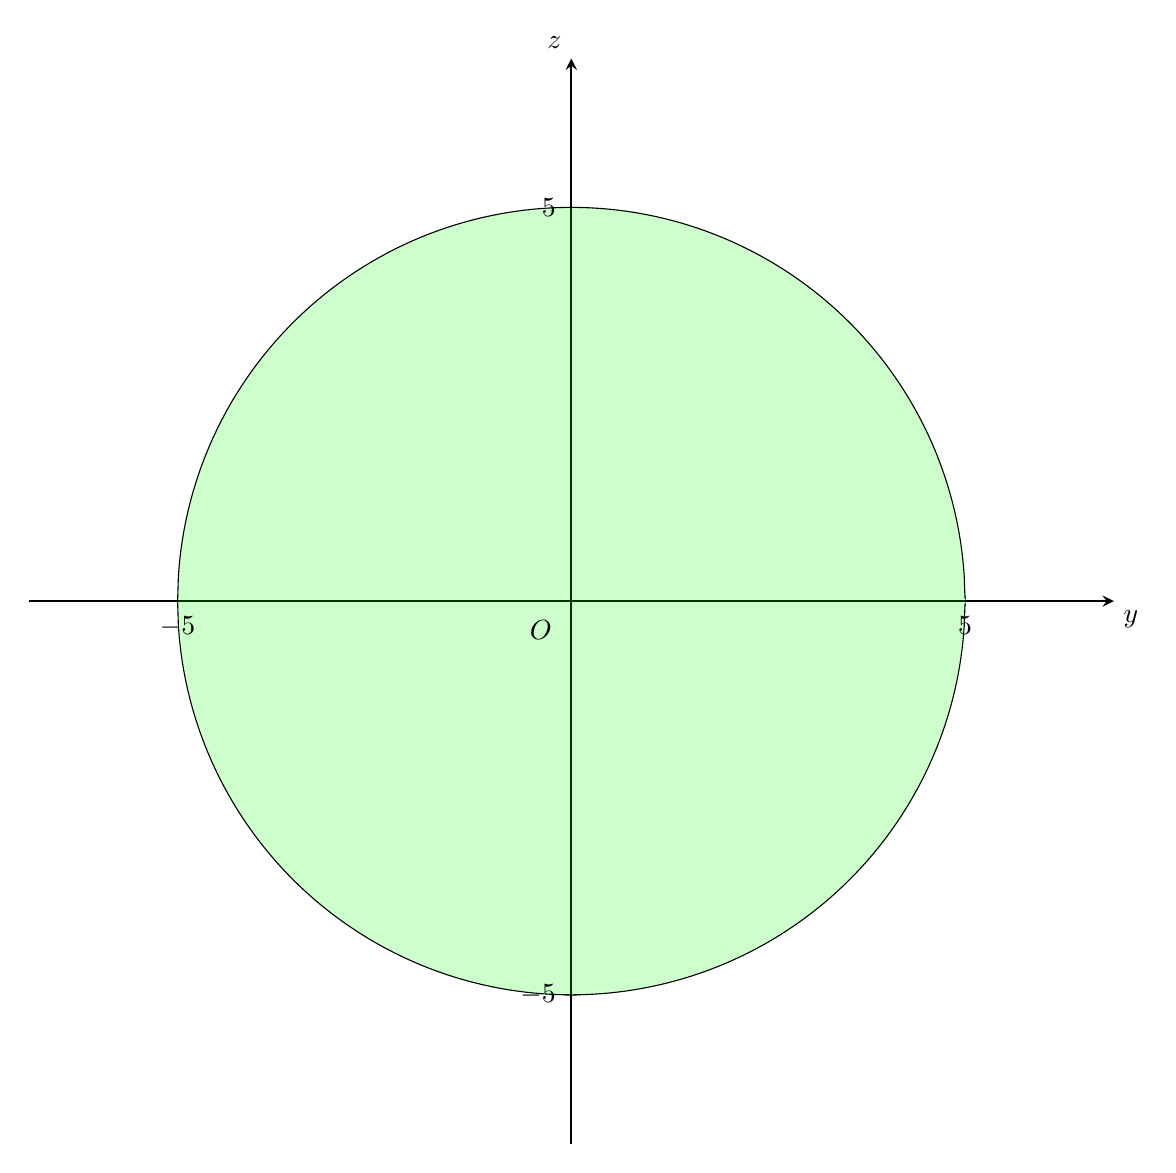
\begin{tikzpicture}
    \begin{axis}[standard,
            xtick={-5,5},
            ytick={-5,5},
            samples=1000,
            xlabel={$y$},
            ylabel={$z$},
          xmin=-5.3,
          xmax=5.3,          
          ymin=-5.3,
          ymax=5.3,
            x=1cm,
            y=1cm/1,
           ]

    \node[anchor=center,label=south west:$O$] at (axis cs:0,0){};
\addplot[name path=F,domain={-5:5}]{sqrt(5^2-x^2)};
\addplot[name path=G,domain={-5:5}]{-sqrt(5^2-x^2)};
\addplot[fill=green, fill opacity=0.2] fill between [of=F and G, soft clip={domain=-5:5}];
    \end{axis}
    \end{tikzpicture}
}
\end{center}
A circle... let's convert the $xy$ region into a polar region. Don't forget that we'll need to throw in our Jacobian $r$ into our integral.

Our lower and upper bounds for $r$ are $r=0$ and $r=4$, respectively.

Our lower and upper bounds for $\theta$ are $\theta=0$ and $\theta=2\pi$, respectively.

In polar, $x=r\cos\theta$, $y=r\sin\theta$, and $z=z$. Therefore,
\begin{align*}
    z&\leq \sqrt{25-(x^2+y^2)}\leq \sqrt{25 - r^2}\tag{in polar, $x^2+y^2=r^2$}\\
    \nabla \cdot \F &=2z\tag{no change}
\end{align*}
Let's evaluate the integral.
\begin{align*}
    \iint_S \F\cdot \n\,d\sigma 
    &=\int_0^{2\pi}\int_0^{4}\int_3^{\sqrt{25-r^2}}2rz\,dz\,dr\,d\theta\tag{don't forget our Jacobian $r$!}\\
    &=\int_0^{2\pi}\int_0^{4}\lrb{rz^2}_3^{\sqrt{25-r^2}}\,dr\,d\theta\\
    &=\int_0^{2\pi}\int_0^4 r\lrp{\sqrt{25-r^2}}^2-r(3)^2\,dr\,d\theta\\
    &=\int_0^{2\pi}\int_0^4 r(25-r^2)-9r\,dr\,d\theta\\
    &=\int_0^{2\pi}\int_0^4 25r-r^3-9r\,dr\,d\theta\\
    &=\int_0^{2\pi}\int_0^4  -r^3 +16r\,dr\,d\theta\\
    &=\int_0^{2\pi}\lrb{-\frac{1}{4}r^4+8r^2}_0^4\,d\theta\\
    &=\int_0^{2\pi}-\frac{1}{4}(4)^4+8(4)^2\,d\theta\\
    &=\int_0^{2\pi}64\,d\theta\tag{use a calculator}\\
    &=\lrb{64\theta}_0^{2\pi}\\
    &=64(2\pi)\\
    &=\boxed{128\pi}
\end{align*}

\phantomsection
\addcontentsline{toc}{section}{Problem 11}\textbf{Problem 11}

Integrate $\F(x,y,z)=\lra{3xz^2,y,-z^3}$ across the surface of the solid in the first octant that is bounded by the cylinder $x^2+4y^2=16$ and the planes $y=2z$, $x=0$, and $z=0$.

\Solution

\textit{Similar problems in Homework 23, Problem 2; Campuswire \#99}

Recall that by Divergence Theorem,
\begin{align*}
    \iint_S \F\cdot \n\,d\sigma &=\iiint_D \nabla \cdot \F\,dV
\end{align*}
Since $\F(x,y,z)=\lra{3xz^2,y,-z^3}$,
\begin{align*}
    \nabla \cdot \F& = \lra{\frac{\partial }{\partial x},\frac{\partial }{\partial y},\frac{\partial }{\partial z}}\cdot \lra{3xz^2,y,-z^3}\\
    &=\frac{\partial }{\partial x}\lrp{3xz^2}+\frac{\partial }{\partial y}\lrp{y}+\frac{\partial }{\partial z}\lrp{-z^3}\\
    &=\lrp{3z^2}+\lrp{1}+\lrp{-3z^2}\\
    &=1
\end{align*}
Let's find the bounds for $D$ in terms of $x$, $y$, and $z$. Don't forget that we're in the first octant so $x,y,z\geq 0$.


Our lower and upper bounds for $z$ are $z=0$ and $z=\dfrac{y}{2}$, respectively. (Since $y=2z$, we know $\dfrac{y}{2}=z$.)

Our lower and upper bounds for $y$ are $y=0$ and $y=\sqrt{4-\dfrac{1}{4}x^2}$, respectively. (Since $x^2+4y^2=16$, we know $4y^2=16-x^2\implies y^2=4-\dfrac{1}{4}x^2$.)

Our lower and upper bounds for $x$ are $x=0$ and $x=4$, respectively. (Since $x^2+4y^2=16$, when $y=0$, $x^2=16\implies x=4$).

Let's evaluate the integral.
\begin{align*}
    \iint_S \F\cdot\n\,d\sigma &=\int_0^4\int_0^{\sqrt{4-\frac{1}{4}x^2}}\int_0^{y/2}1\,dz\,dy\,dx\\
    &=\int_0^4\int_0^{\sqrt{4-\frac{1}{4}x^2}}\lrb{z}_0^{y/2}\,dy\,dx\\
    &=\int_0^4\int_0^{\sqrt{4-\frac{1}{4}x^2}}\frac{y}{2}\,dy\,dx\\
    &=\int_0^4\lrb{\frac{1}{4}y^2}_0^{\sqrt{4-\frac{1}{4}x^2}}\,dx\\
    &=\int_0^4 \frac{1}{4}\lrp{\sqrt{4-\frac{1}{4}x^2}}^2\,dx\\
    &=\int_0^4 \frac{1}{4}\lrp{4-\frac{1}{4}x^2}\,dx\\
    &=\int_0^4 1 - \frac{1}{16}x^2\,dx\\
    &=\lrb{x-\frac{1}{48}x^3}_0^4\\
    &=4-\frac{1}{48}(4)^3\\
    &=\boxed{\frac{8}{3}}\tag{use a calculator}
\end{align*}
\phantomsection
\addcontentsline{toc}{section}{Problem 12}\textbf{Problem 12}

The state of Wyoming is bounded by the meridians $111\degree3'$ and $104\degree3'$ west longitude and by the circles $41\degree$ and $45\degree$ north latitude. Assuming that the Earth is a sphere of radius $3959$ mi, find the area of Wyoming. (\textit{Hint}: Use the modified spherical coordinates from problem 4 of Homework 17.)

\Solution

\textit{Similar problems in Homework 17, Problem 2 and Problem 4; Campuswire \#64 }

Since the Earth is a sphere of radius $3959$ mi, let's have our surface be represented as $x^2+y^2+z^2=3959^2$.

\textit{Sphere}... let's use spherical coordinates to parameterize our surface!

We'll be using a slightly modified version of spherical coordinates so that we can have one of our angles ($\psi=\dfrac{\pi}{2}-\phi$) be measured up from the $xy$-plane (equator) instead of down from the $z$-axis (north pole).
\begin{center}
\resizebox{6cm}{!}{
\tikzset{every picture/.style={line width=0.75pt}} %set default line width to 0.75pt        

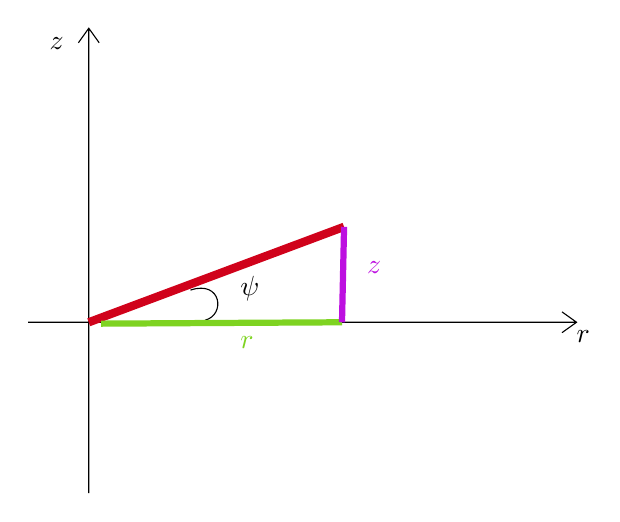
\begin{tikzpicture}[x=0.75pt,y=0.75pt,yscale=-1,xscale=1]
%uncomment if require: \path (0,300); %set diagram left start at 0, and has height of 300

%Shape: Axis 2D [id:dp3868879526535256] 
\draw  (212,174.67) -- (476.17,174.67)(241.17,33) -- (241.17,257) (469.17,169.67) -- (476.17,174.67) -- (469.17,179.67) (236.17,40) -- (241.17,33) -- (246.17,40)  ;
%Curve Lines [id:da7616688363692427] 
\draw    (297.17,173.67) .. controls (307.17,171.17) and (305.17,154.17) .. (290.17,159.17) ;
%Straight Lines [id:da9959122238211519] 
\draw [color={rgb, 255:red, 208; green, 2; blue, 27 }  ,draw opacity=1 ][line width=3]    (241.17,174.67) -- (364.17,128.67) ;
%Straight Lines [id:da8585096856285587] 
\draw [color={rgb, 255:red, 126; green, 211; blue, 33 }  ,draw opacity=1 ][line width=2.25]    (247.17,175.33) -- (363.17,174.67) ;
%Straight Lines [id:da05876942804651064] 
\draw [color={rgb, 255:red, 189; green, 16; blue, 224 }  ,draw opacity=1 ][line width=2.25]    (364.17,128.67) -- (363.17,174.67) ;

% Text Node
\draw (221,36.4) node [anchor=north west][inner sep=0.75pt]    {$z$};
% Text Node
\draw (475,177.4) node [anchor=north west][inner sep=0.75pt]    {$r$};
% Text Node
\draw (313,151.4) node [anchor=north west][inner sep=0.75pt]    {$\psi $};
% Text Node
\draw (313,180.4) node [anchor=north west][inner sep=0.75pt]  [color={rgb, 255:red, 126; green, 211; blue, 33 }  ,opacity=1 ]  {$r$};
% Text Node
\draw (374,144.4) node [anchor=north west][inner sep=0.75pt]  [color={rgb, 255:red, 189; green, 16; blue, 224 }  ,opacity=1 ]  {$z$};


\end{tikzpicture}}
\end{center}
(the red line is our radius, $3959$)

In our modified spherical coordinate system,
\begin{align*}
    x&=3959\cos\psi\cos\theta\tag{$r=3959\cos\psi$}\\
    y&=3959\cos\psi\sin\theta\tag{$r=3959\cos\psi$}\\
    z&=3959\sin\psi
\end{align*}
Let's find the bounds for $\psi$ and $\theta$.

For $\psi$,

Since we're bounded by $41\degree$ and $45\degree$ north latitude, 
\begin{equation*}
    \frac{41\pi}{180}\leq  \psi \leq \frac{45\pi}{180}\tag{$\displaystyle1\degree = \frac{\pi}{180\degree}$}
\end{equation*}
For $\theta$,

Since we're bounded by $111\degree3'$ and $104\degree3'$ west longitude,
\begin{equation*}
    \frac{104.3\pi}{180}\leq \theta\leq \frac{111.3\pi}{180}\tag{$\displaystyle1\degree = \frac{\pi}{180\degree}$}
\end{equation*}
Therefore, our parameterization is
\begin{equation*}
    \r\lrp{\psi, \theta}=\lra{3959\cos\psi\cos\theta, 3959\cos\psi\sin\theta, 3959\sin\psi}
\end{equation*}
where $\displaystyle\frac{41\pi}{180}\leq  \psi \leq \frac{45\pi}{180}$ and $ \displaystyle\frac{104.3\pi}{180}\leq \theta\leq \frac{111.3\pi}{180}$.

\textbf{Surface Area}

Now that we have our parameterization, let's calculate the surface area.

Recall that surface area is
\begin{align*}
    S=\iint_R \norm{\frac{\partial \r}{\partial u}\times \frac{\partial \r}{\partial v}}\,dA
\end{align*}
Let's have $u=\psi$ and $v=\theta$.

Let's find what $\displaystyle \norm{\frac{\partial \r}{\partial \psi}\times \frac{\partial \r}{\partial \theta}}$ is. 

Since $ \r\lrp{\psi, \theta}=\lra{3959\cos\psi\cos\theta, 3959\cos\psi\sin\theta, 3959\sin\psi}$,
\begin{align*}
    \frac{\partial \r}{\partial \psi}&=\lra{-3959\sin\psi\cos\theta, -3959\sin\psi\sin\theta, 3959\cos\psi}\\
    \frac{\partial \r}{\partial \theta}&=\lra{-3959\cos\psi\sin\theta, 3959\cos\psi\cos\theta, 0}\\
      \frac{\partial \r}{\partial \psi}\times   \frac{\partial \r}{\partial \theta}&=\begin{vmatrix}\i & \j & \k\\ -3959\sin\psi\cos\theta& -3959\sin\psi\sin\theta& 3959\cos\psi\\-3959\cos\psi\sin\theta& 3959\cos\psi\cos\theta& 0\end{vmatrix}\\
      &=\lrp{0-3959^2\cos^2\psi\cos\theta}\i-\lrp{0+3959^2\cos^2\psi\sin\theta}\j + \lrp{-3959^2\sin\psi\cos\psi\cos^2\theta-3959^2\sin\psi\cos\psi\sin^2\theta}\k\\
      &=\lrp{-3959^2\cos^2\psi\cos\theta}\i-\lrp{3959^2\cos^2\psi\sin\theta}\j+\lrp{-3959^2\sin\psi\cos\psi\lrp{\cos^2\theta+\sin^2\theta}}\k\\
      &=\lrp{-3959^2\cos^2\psi\cos\theta}\i-\lrp{3959^2\cos^2\psi\sin\theta}\j+\lrp{-3959^2\sin\psi\cos\psi}\k\tag{$\cos^2\theta+\sin^2\theta=1$}\\
      &=\lra{-3959^2\cos^2\psi\cos\theta,-3959^2\cos^2\psi\sin\theta, -3959^2\sin\psi\cos\psi}\\
      \norm{ \frac{\partial \r}{\partial \psi}\times   \frac{\partial \r}{\partial \theta}}&=\sqrt{3959^4\cos^4\psi\cos^2\theta+3959^4\cos^4\sin^2\theta+3959^4\sin^2\psi\cos^2\psi}\\
      &=\sqrt{3959^4\cos^4\psi\lrp{\cos^2\theta+\sin^2\theta}+3959^4\sin^2\psi\cos^2\psi}\\
      &=\sqrt{3959^4\cos^4\psi+3959^4\sin^2\phi\cos^2\psi}\tag{$\cos^2\theta+\sin^2\theta$}\\
      &=\sqrt{3959^4\cos^2\psi\lrp{\cos^2\psi + \sin^2\psi}}\\
      &=\sqrt{3959^4\cos^2\psi}\tag{$\cos^2\psi + \sin^2\psi = 1$}\\
      &=3959^2\cos\psi\tag{ok to drop abs since $41\degree \leq \psi \leq 45\degree$}
\end{align*}
Let's evaluate the integral.
\begin{align*}
    S&=\int_{104.3\pi/180}^{111.3\pi/180}\int_{41\pi/180}^{45\pi/180}3959^2\cos\psi\,d\psi\,d\theta\\
    &=\int_{104.3\pi/180}^{111.3\pi/180}\lrb{3959^2\sin\psi}_{41\pi/180}^{45\pi/180}\,d\theta\\
    &=\int_{104.3\pi/180}^{111.3\pi/180}3959^2\sin\frac{45\pi}{180}-3959^2\sin\frac{41\pi}{180}\,d\theta\\
    &=\lrb{\lrp{3959^2\sin\frac{45\pi}{180}-3959^2\sin\frac{41\pi}{180}}\theta}_{104.3\pi/180}^{111.3\pi/180}\\
    &=\lrp{3959^2\sin\frac{45\pi}{180}-3959^2\sin\frac{41\pi}{180}}\lrp{\frac{111.3\pi}{180}}-\lrp{3959^2\sin\frac{45\pi}{180}-3959^2\sin\frac{41\pi}{180}}\lrp{\frac{104.3\pi}{180}}\\
    &=\lrp{3959^2\sin\frac{45\pi}{180}-3959^2\sin\frac{41\pi}{180}}\lrp{\frac{111.3\pi}{180}-\frac{104.3\pi}{180}}\\
    &=\lrp{3959^2\sin\frac{45\pi}{180}-3959^2\sin\frac{41\pi}{180}}\lrp{\frac{7\pi}{180}}\\
    &=\boxed{\lrp{3959^2}\lrp{\sin\frac{45\pi}{180}-\sin\frac{41\pi}{180}}\lrp{\frac{7\pi}{180}}\text{mi}^2\approx97,751.41\text{mi}^2}\tag{use a calculator}
\end{align*}
\end{document}
